\documentclass{article} % For LaTeX2e
\usepackage{nips14submit_e,times}
\usepackage{hyperref}
\usepackage{url}
\usepackage{amsmath,amssymb}
\usepackage{graphicx}
\usepackage[T1]{fontenc}
%\usepackage{babel}



%\documentstyle[nips14submit_09,times,art10]{article} % For LaTeX 2.09


\author{
Stephanie deWet \\
Department of Computer Sciences\\
University of Wisconsin - Madison \\
Madison, WI 53705 \\
\texttt{sdewet@cs.wisc.edu} \\
\and
Saswati De \\
Department of Computer Sciences\\
University of Wisconsin - Madison \\
Madison, WI 53705 \\
\texttt{sde@cs.wisc.edu} \\
}

\title{Applying Gaussian Process Regression to Predict Changes in Stock Price}


\newcommand{\fix}{\marginpar{FIX}}
\newcommand{\new}{\marginpar{NEW}}

%\nipsfinalcopy % Uncomment for camera-ready version

\def\bfx{\mathbf x}
\def\bfy{\mathbf y}
\def\bftheta{\mathbf \theta}
\def\bfl{\mathbf \mathcal l}
\def\l{\mathcal l}
\def\R{\mathbb R}
\def\diag{\mbox{ diag }}



\begin{document}


\maketitle

\begin{abstract}
Predicting stock prices is an interesting problem for machine learning researchers. In this paper we use Gaussian Processes to model the timeseries representing the change in price of a single stock. Our implementation of the GP model performed well in comparison to other regression models like Linear Regression and PCA Regression.
\end{abstract}

\section{Introduction}
In stock markets, investors need long-term forecasting techniques to choose the right time to buy/sell stocks to maximize their profits or to minimize their loss. The majority of existing stock market forecasting techniques rely on machine learning tools and the accuracy of these tools is still a significant challenge for market traders considering the several external factors which affect the stock market. In this project we have tried to forecast change in stock price using the Gaussian Processes (GP) model.

\section{Initial Data Processing}
Our data set (obtained from [4]) consists of information collected on a single stock, including instantaneous stock prices and instantaneous values of 27 parameters ($P$) known to have some effect on the price.
These values are taken at many different time stamps.
Our goal is to predict the stock price in the near future, given current values of the parameters.

First, we create labeled data to use in training our models using the following process:
We sort the data set in increasing time.
For each line, we define $\delta$, the difference in stock price after \textbf{t} milliseconds, to be the current stock price subtracted from the stock price that is closest to \textbf{t} milliseconds in the future.
%(Note that our datapoints are close enough together that the difference in time between sets of data points will be much less than modeling error.)
We will attempt to build a model which calculates $\delta_t$ when given $P_t$, the values of the 27 parameters at time $t$.

% Note to self: this is done in strategy 

% TODO:  Insert a paragraph about normalization of data.


\section{Algorithm}

Our algorithm could be divided into 5 major parts - preprocessing the data, building the covariance matrix, tuning the hyperparameters, learning the GP model using a windowing technique and finally predicting the change in stock price for the next time instance using the learned GP model. 

\subsection{Pre-processing}
\label{sec:strategy}

We experiment with 3 different strategies to build our training set from the available dataset. In the first strategy we prune out all data points that were more than one standard deviation \textbf{away} from the sample mean $\bf\bar{y}$. In the second strategy we prune out all data points that were \textbf{within} one standard deviation from the sample mean $\bf\bar{y}$. And for the third strategy, we keep all data points. After applying any one of the above strategies to the data, we linearly scale the inputs to have zero mean and unit variance on the training set. We also centered the corresponding target outputs so as to have zero mean on the training set.

\subsection{Building the Covariance Matrix}

We initially build the covariance matrix $K$ using the first $\mathcal{T}$ samples, i.e using the samples from $t = 0$ to $t = \mathcal{T}$. While building $K$, we have experimented with a few interesting covariance functions as described below:  

\subsubsection{Covariance Functions}
We consider 4 different covariance functions, all of which can be parameterized in terms of the hyperparameters $\bftheta = \{\bfl, \sigma_n^2 \sigma_f^2\}$, where $\bfl$ is a length 27 vector.
Let
\begin{equation}
	u = \left( \left( \bfx_p - \bfx_q \right)^\top \diag(\bfl)^{-2} \left( \bfx_p - \bfx_q \right) \right)^{1/2}
\end{equation}

Then, the covariance functions are:
\begin{align}
	k(\bfx_p, \bfx_q) &= \sigma_f^2 \exp\{- \frac{1}{2} u^2\} + \sigma_n \delta_{pq} \quad \quad \quad \mbox{(Squared Exponential)}   \\
	k(\bfx_p, \bfx_q) &= \sigma_f^2 \exp\{- u\} + \sigma_n \delta_{pq} \quad \quad \quad \mbox{(Ornstein Uhlenbeck)}   \\
	k(\bfx_p, \bfx_q) &= \sigma_f^2 \left( 1 + \sqrt{3} u \right) \exp\{- \sqrt{3}  u\} + \sigma_n \delta_{pq} \quad \quad \quad \mbox{(Matern - $\nu = \frac{3}{2}$)}   \\
	k(\bfx_p, \bfx_q) &= \sigma_f^2 \left( 1 + \sqrt{5} u \right) + 5 u^2) \exp\{- \sqrt{5} u\} + \sigma_n \delta_{pq} \quad \quad \quad \mbox{(Matern  - $\nu = \frac{5}{2}$)}
\end{align}

$\sigma_n^2$ and $\sigma_f^2$ are the noise and signal level parameters, respectively, and $l_1, \dots, l_D$ are characteristic length-scales.
The covariance matrix $K_y$ is given by $[K_y]_{pq} = k(\bfx_p, \bfx_q)$.
We can think of these length-scales as a measure of the irrelevance of the associated feature; a large value of $l_i$ means that the $i$-th parameter of the feature vector has very little effect on the resultant covariance matrix.
This is a type of automatic relevance determination (ARD).


\subsection{Tuning the hyperparameters}
For the covariance matrices above, we tuned the hyperparameters by maximizing the log marginal likelihood, 
\begin{equation}
	\log p(\bfy | X, \bftheta) = - \frac{1}{2} \bfy^\top K_y^{-1} \bfy - \frac{1}{2} \log | K_y | - \frac{n}{2} \log (2 \pi)
\end{equation}

Rasmussen and Williams state that the maximum of this quantity is generally more pronounced for larger numbers of data points.
They also note that this function is not concave, and so there could be multiple local optima.
However, they suggest that for larger data sets, one local optimum will generally be orders of magnitude more probable than the others, and that this can generally be assumed to be the correct choice of hyperparameters.

For all except the exponential function, we calculate the gradient $\frac{\partial K} {\partial \bftheta}$ and use a gradient-based descent method.
Note that $K_y \in \R^{n \times n}$ must be recalculated at each step of the optimization.
As the size of the data set grows, this becomes increasingly intractable.
Therefore, we follow the suggestion of Rasmussen \& Williams in their example (Ch 2), and optimize the hyperparameters based on a smaller subset of the data.

We calculated the marginal likelihood using the first 500 data points from the training set, and also using 500 random data points from the training set.
We found that the K matrix was ill-conditioned when we used 500 random data points, so we did not use these values in our experiments.
Ideally, we would have used a larger dataset and more random restarts, but we were unable to do so due to time constraints.
We believe this is one of the major sources of error in our project.
After we obtain the optimized set of hyperparameters, the same set is employed in all our experiments.

We also observed that the resultant $\bfl$ parameters had very large values in the majority of their coefficients and smaller values for a limited subset of components.
This means that a limited number of components have a larger correlation with the target value.


\subsection{Learning the GP Model}

We have applied a windowing technique to learn a GP on the data. We use the covariance matrix built using data from $t = 0$ to $t = \mathcal{T}$, to predict the change in stock price at time $t = \mathcal{T}+1$. Once the prediction is made, we use the input vector at $t = \mathcal{T}+1$ and the \textbf{\textit{predicted}} change in price at that instance as a new data point and compute the covariance matrix again for the window from $t = 1$ to $t = \mathcal{T}+1$. We use this newly computed covariance matrix to predict the change in stock price at $t=\mathcal{T}+2$. This process is repeated until $t = \mathcal{T}+T$, where $T$ denotes how far ahead in future we want to keep predicting the change in stock prices.

Since re-computing the covariance matrix for every window can be time consuming, we compute only the last column / row of the covariance matrix as it corresponds to the time instance $t = \mathcal{T}+1$. In addition, we drop the row and column that correspond to the oldest time instance of the previous window, from the covariance matrix. We repeat this procedure for every new $t$ that we predict. This keeps the size of our covariance matrix constant (therefore, keeping the amount of computation required for inverting the covariance matrix constant across every window) while allowing us to re-use the other columns of the covariance matrix that correspond to the time instances common to the previous window and the current window.

\subsection{Prediction}

We predict the change in stock price at the time instance immediately following our current time window, to be the \textbf{\textit{mean}} of the below conditional distribution:

\begin{equation}
 \boldsymbol{f_*} | \boldsymbol{X}, \boldsymbol{y}, \boldsymbol{X_*} \sim \mathcal{N}\left(\bar{\boldsymbol{f_*}}, \mbox{cov}(\boldsymbol{f_*})\right)
\end{equation}
where,
\begin{align}
\bar{\boldsymbol{f_*}} &= \boldsymbol{K}\left(\boldsymbol{X_*}, \boldsymbol{X}\right) \left[ \boldsymbol{K}\left(\boldsymbol{X}, \boldsymbol{X}\right) + \sigma_n^2\boldsymbol{I}\right]^{-1} \boldsymbol{y} \\
\mbox{cov}(\boldsymbol{f_*}) &= \boldsymbol{K}\left(\boldsymbol{X_*}, \boldsymbol{X_*}\right) - \boldsymbol{K}\left(\boldsymbol{X_*}, \boldsymbol{X}\right) \left[ \boldsymbol{K}\left(\boldsymbol{X}, \boldsymbol{X}\right) + \sigma_n^2\boldsymbol{I}\right]^{-1} \boldsymbol{K}\left(\boldsymbol{X}, \boldsymbol{X_*}\right)
\end{align}

Finally we scale the predicted value back by adding the sample mean - $\bf\bar{y}$, of the target vector to our prediction.

\section{Experiments}

\subsection{Covariance Type}
For this experiment, we use $\mathcal{T} = 20000$, with Strategy 3, and try to predict 500 ms into the future.
In figure \ref{fig1}, we found that squared exponential, Ornstein Uhlenbeck and the Matern function with $\nu = \frac{5}{2}$ predicted nearly a straight line, with very small variations.
The Matern function with $\nu = \frac{3}{2}$ had predictions shaped more like the actual data, with sharp peaks and valleys.

\begin{figure}[h]
	\label{fig1}
	\centering
	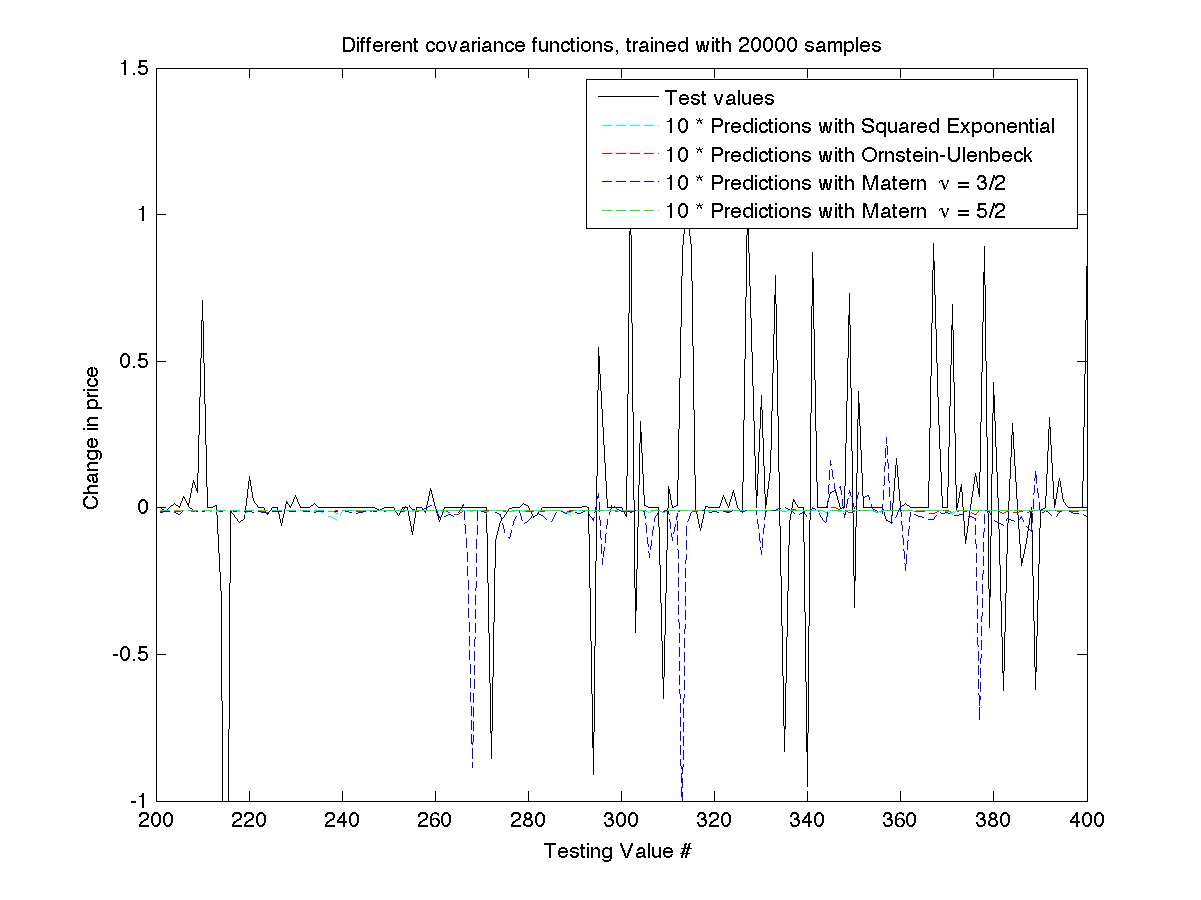
\includegraphics[width=0.8\textwidth]{../code/fig_1.png}
	\caption{Covariance Functions Experiment}
\end{figure}

The Matern function with $\nu = \frac{3}{2}$ looked most like the data, but the Ornstein-Uhlenbeck model had a smaller mean squared error, so we used it for all future experiments.

\subsection{Window size}
Next, we experimented with varying window size $\mathcal{T}$, while using Strategy 3 and predicting 500 ms into the future.
In figure \ref{fig2}, we found that the larger windows predicted the dominant trend much better, and had fewer peaks and valleys.

\begin{figure}[h]
	\label{fig2}
	\centering
	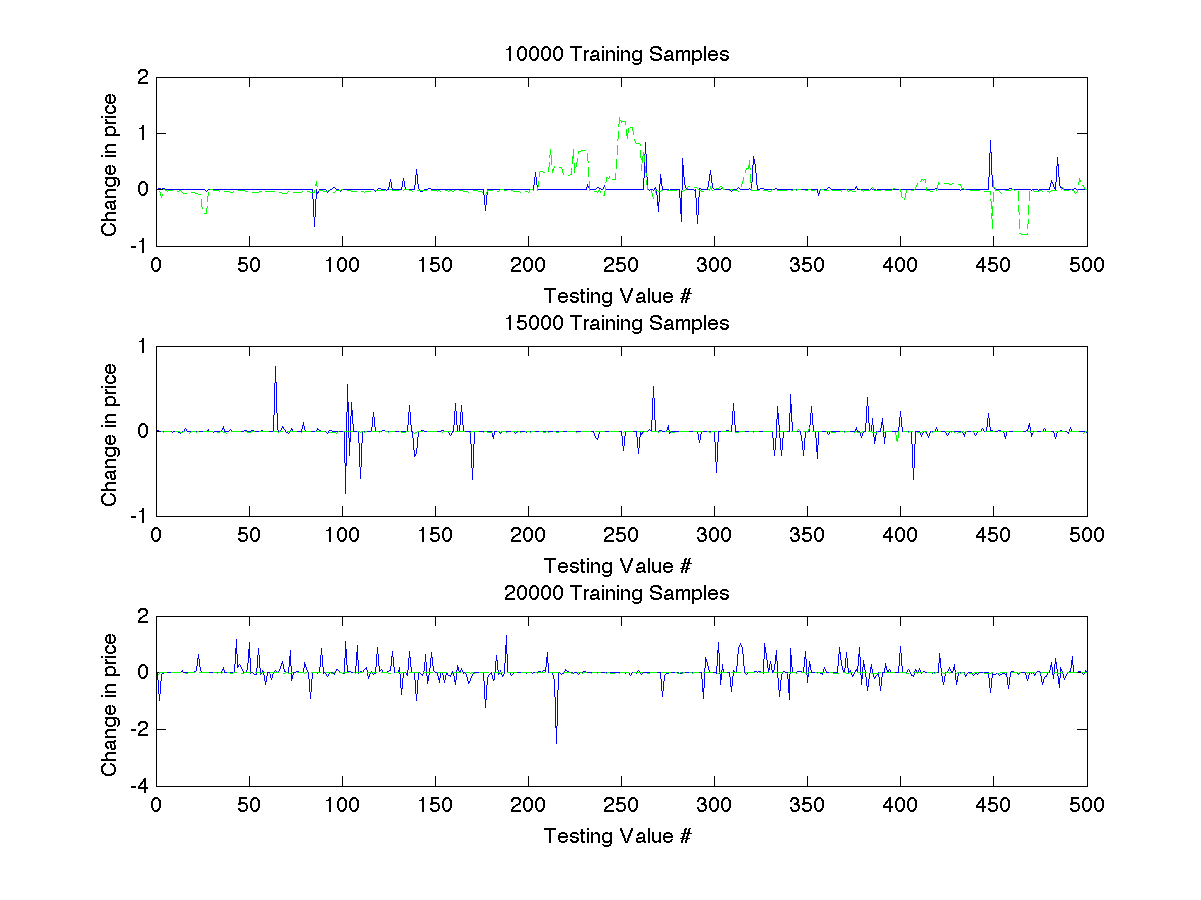
\includegraphics[width=0.8\textwidth]{../code/fig_2.png}
	\caption{Window Experiments}
\end{figure}

\subsection{Strategy Type}
We tried several different strategies (described in \ref{sec:strategy}).
We then applied an earnings predictor, provided with [4], to our predicted values.
The earnings of a model measure how well it fits the dataset.
\begin{table}[h]
	\label{t}
	\centering
	\caption{Earnings from different strategies}
	\begin{tabular}{| l | l |}
	\hline
	Strategy & Earnings \\
	\hline
	1 & 42.88 \\
	2 & 28.39 \\
	3 & 3.86 \\
	\hline
	\end{tabular}
\end{table}

In table \ref{t}, we found that breaking the data into inliers and outliers helped us to predict the trend much better.
We think this is because these models had less variation and were easier to train.
With more training data and time, the Strategy 0 model may have done better too.


\subsection{Future time}
In experiments up to this point, we used data that had been processed so that the y values are the change in stock price 500 ms in the future.
Next, we re-processed the data to have y values 800 ms or 1000 ms in the future.
We found that we got roughly the same results for each experiment, suggesting that we are equally capable of predicting on each of these time scales into the future.

If we had more time, we would run additional experiments further into the future, to see how far ahead we can predict before our model's performance gets notably worse.
We also discovered that the data does not have a high enough precision.  In many cases, the stock prices aren't given to enough decimal places, so the change in price is just 0.
Using larger time gaps might have helped to ameliorate this problem.


\subsection{Comparisons to other models}
The dataset that we used came with pre-trained linear regression and PCA regression models.
In Figure \ref{fig4}, we show comparisons of earnings of the different learning algorithms.  Each group of bars is tested on the same set of data.

\begin{figure}[h]
	\label{fig4}
	\centering
	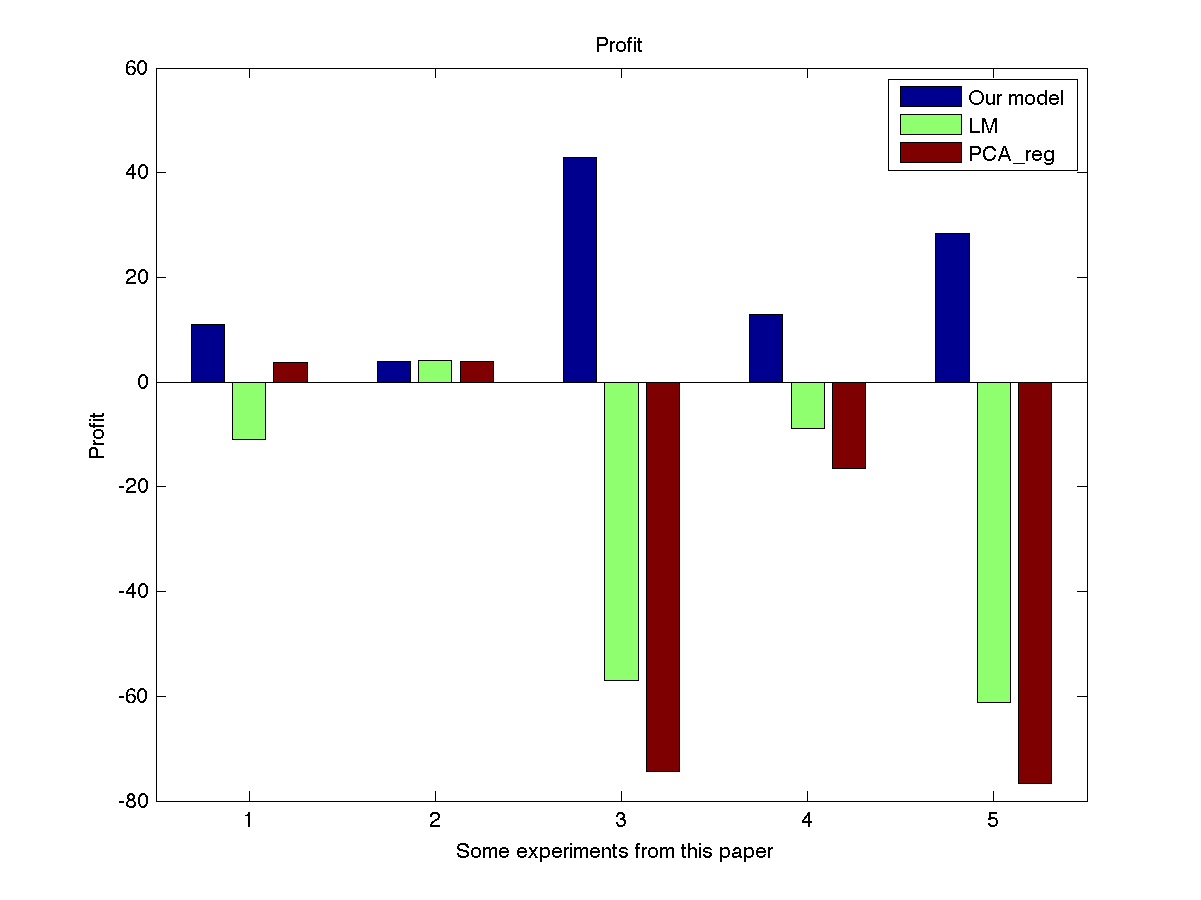
\includegraphics[width=0.8\textwidth]{../code/fig_4.png}
	\caption{Comparisons Between Different Learning Algorithms}
\end{figure}

\section{Conclusion}
The results from our experiments indicate that GP models could learn the correlations hidden among financial data to a very high degree when compared to other traditional ML algorithms like linear regression and PCA regression. But the biggest drawback of GP models as implemented in our application is the computation time that is required for the GP modeling. Regression based on GP models involve a huge amount of matrix inversions, the complexity of which is to the order of $\mathcal{O}(n^3)$. These computational needs, restricted the amount of training data that could be used, to a maximum of only 20000 training samples, even though we had access to around 2GB of stock price data that we would have liked to use during training. Several authors have suggested sparse approximation approaches for calculating the covariance matrix, which we believe is a promising direction for future work.
Another improvement would be to select the predicted values by sampling from the distribution, rather than using the distribution mean.

\subsubsection*{Contributions}
Saswati contributed the experiment design and the Gaussian Processes code.
Stephanie contributed the covariance optimization code.
Both team members ran experiments, contributed to the paper, and researched the models and methods to be used.

\subsubsection*{Acknowledgments}
Thanks to Prof. Zhu for an excellent class.

\subsubsection*{References}
\small{
	[1] C.E. Rasmussen \& C.K.I. Williams, Gaussian Processes for Machine Learning.

	[2] David Mackay, Introduction to Gaussian Processes.

 [3] Long-term Stock Market Forecasting using Gaussian Processes, Nando de Freitas.

 [4] Dataset - http://www.tworoads.co.in/trading-competition
 }


\end{document}
